\chapter{Implementation}
\label{chap:implementation}


This chapter describes how the architecture of Chapter~\ref{chap:architecture} was built. It opens with the technology choices and their rationale, then works through the components that carry the most design weight: the single point through which every \gls{llm} call passes, the System One classifier and its floor, the payload library and its \glsdisp{filter_evasion}{filter-evasion} layer, attack synthesis and execution, the dual evaluation, the \gls{oauth} flow for authenticated servers, the static analysis engine, the persistence layer, and the test and continuous-integration setup.

\section{Technology Stack}
\label{sec:stack}

The backend is written in Python with FastAPI. The choice is driven by the workload: \gls{mcp} sessions, \gls{llm} calls, and tool calls are all I/O-bound and mostly run concurrently, so an async-native framework fits naturally, and FastAPI produces an OpenAPI description for free. The frontend is a React application built with Vite, using plain \texttt{fetch} and no additional libraries. It runs in the browser and talks to the backend over \gls{http}, which is what the \gls{oauth} flow needs: a server-side interface running inside a container cannot open a login page in the user's own browser, whereas a browser-based frontend can.

Durable scan history is kept in PostgreSQL, accessed through async SQLAlchemy and \texttt{asyncpg}. \gls{json} columns store snapshots, categorizations, and reports without a rigid schema, which suits structures that are still evolving. The \gls{mcp} client is the official \texttt{mcp} Python \gls{sdk} rather than a hand-rolled \gls{jsonrpc} implementation~\cite{anthropic2024mcp}, since the reference implementation already covers the three transports and is actively maintained. Tool classification calls TypeSafe's Jev \gls{api} \citep{typesafe2026systemone}. The \gls{llm} used for attack synthesis and judging is pluggable across OpenAI, Anthropic, and Ollama. Ollama keeps synthesis and judging on the local machine, at some cost to quality, but a scan is not fully offline, since classification still calls Jev's hosted service. Testing uses Pytest with \texttt{pytest-asyncio}. Static analysis of the servers under test combines Python's \texttt{ast} module with Bandit, and the same three tools, Bandit, \texttt{pip-audit}, and \texttt{detect-secrets}, run in continuous integration against the tool's own code on every push.

The three pieces, frontend, backend, and database, run as separate Docker
Compose services, as Figure~\ref{fig:deploy} shows.

\begin{figure}[htbp]
    \centering
    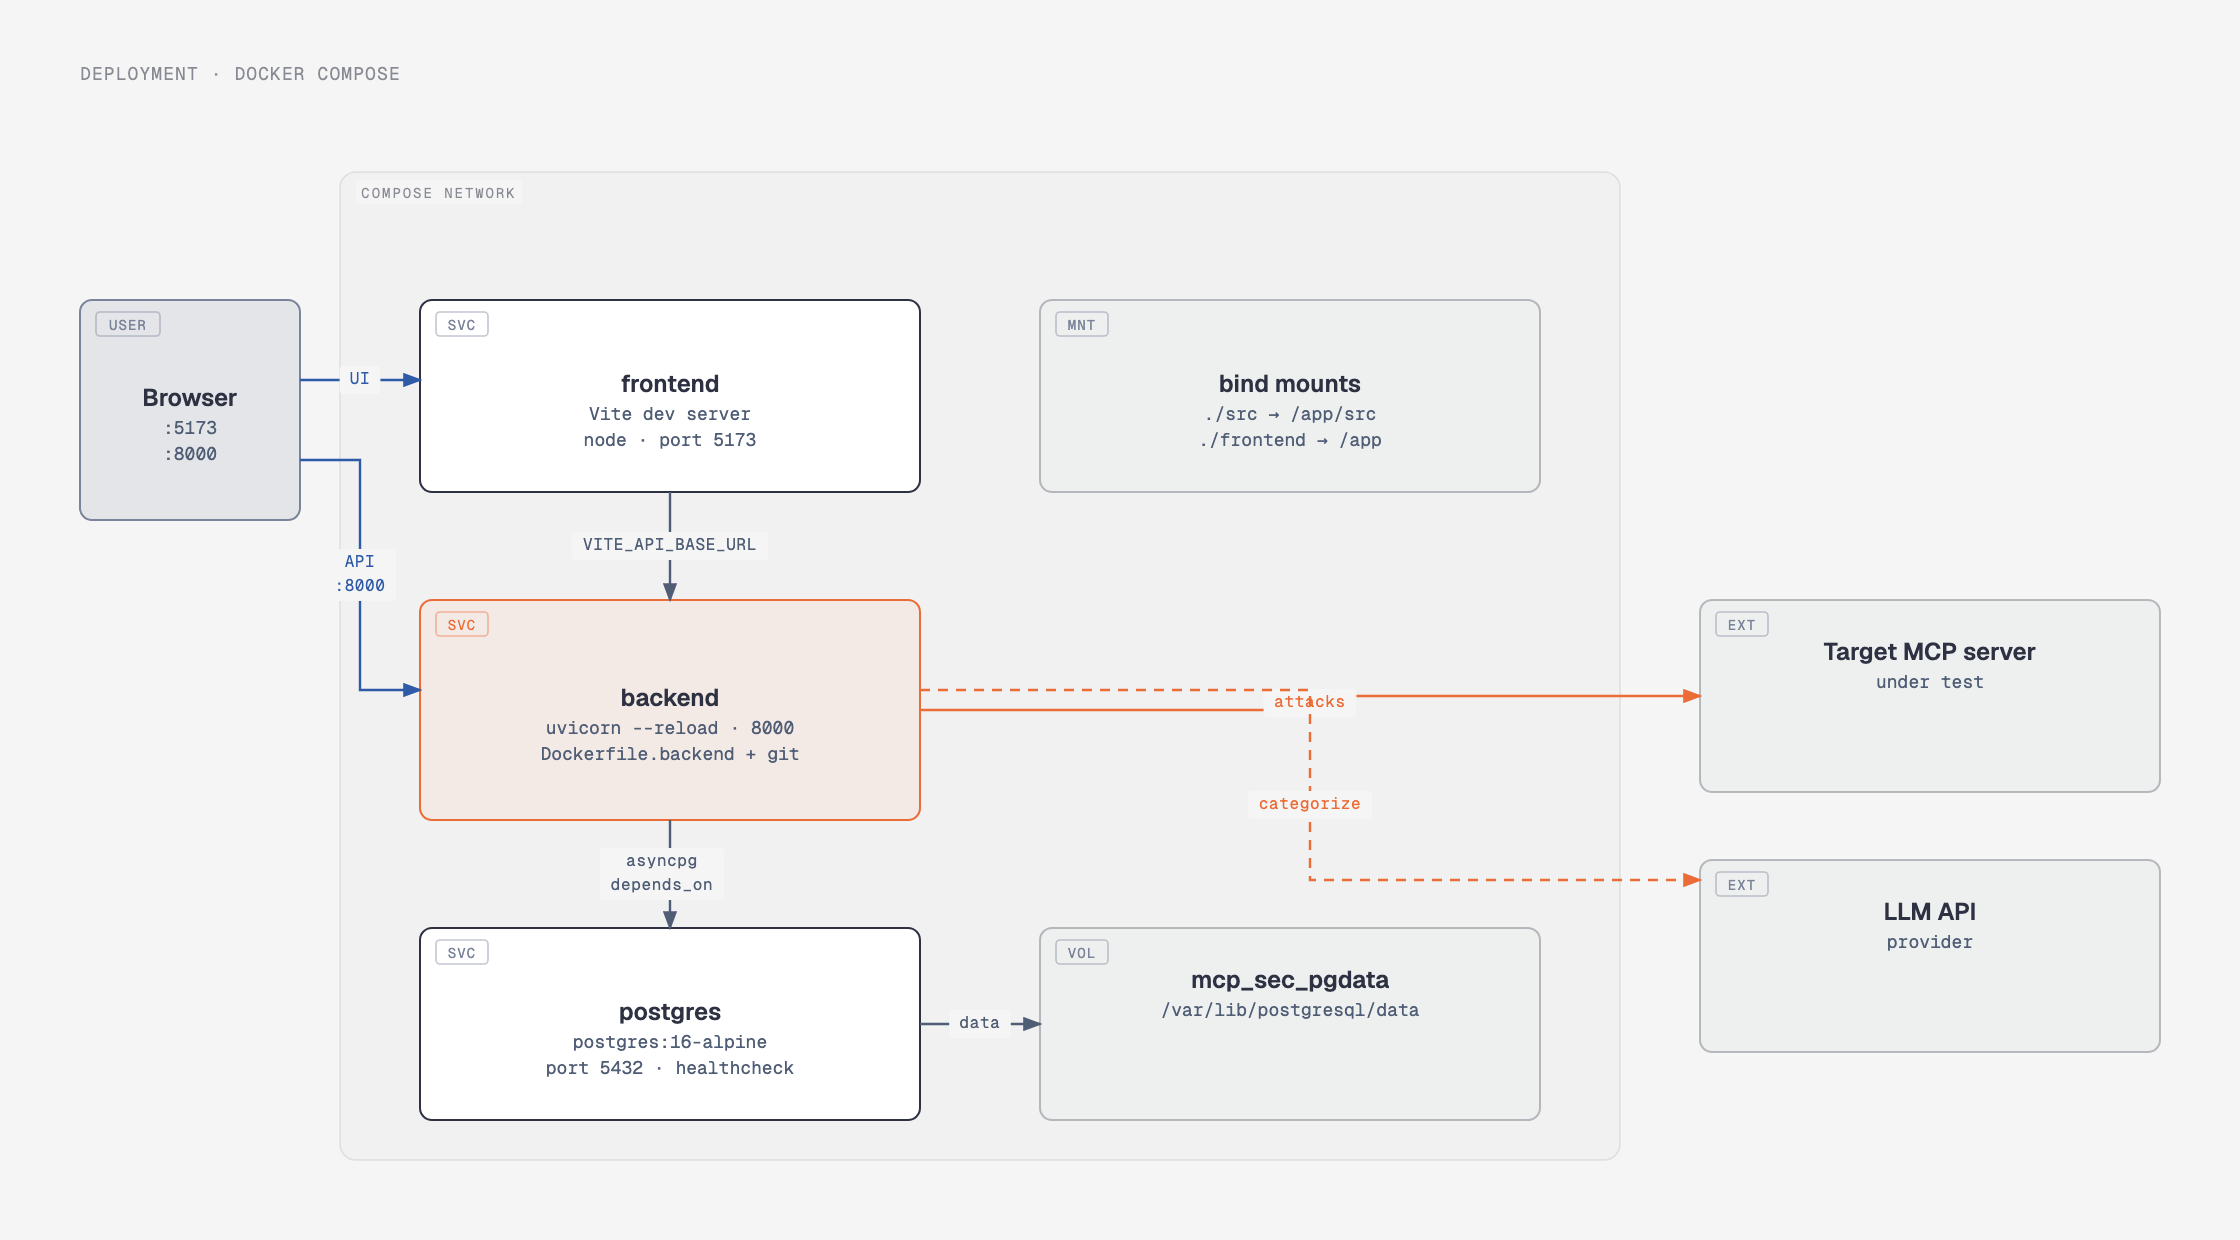
\includegraphics[width=\linewidth]{images/deploy-containers.png}
    \caption{Deployment: the three Docker Compose services, their host port
    mappings, the database volume, and the external target server and LLM API.}
    \label{fig:deploy}
\end{figure}

\section{The LLM Provider Abstraction and Observability}
\label{sec:llm-provider}

Every \gls{llm} call in the pipeline, attack synthesis and judging, passes through one method on a provider abstraction, \texttt{complete\_json}. Each provider implements that method, and each implementation is wrapped in a single tracing decorator. The payoff is twofold. A change to tracing is made once and applies to all three providers uniformly, including Ollama's raw HTTP path, which vendor-specific auto-instrumentation would have missed. And the one chokepoint is where model name and token usage are recorded, which is what later lets the cost of a scan be attributed per call.

The per-call records are grouped into one trace per scan. A scan opens a root span tagged with the target and the provider, and a child span per tool, so an entire scan reads as one tree, discover, categorize, then synthesize and judge for each tool, rather than a hundred disconnected calls. Tracing is a strict no-op when its keys are unset, and every traced call is wrapped so that a tracing fault can never break a scan. This keeps observability genuinely optional: a developer who sets no keys sees no behavioral change at all. Jev requests do not pass through the provider abstraction, since they use a different \gls{api}, but each one is recorded in the same trace with its request, response, and token usage.

\section{Classification with Jev and the Baseline Floor}
\label{sec:categorizer}

The classifier sends Jev each discovered tool's name, description, and input schema as the request state, together with one yes/no question per semantic category, eleven in all, grouped into requests of at most eight questions. Each question carries the category's description and instructs the model to treat the tool definition as untrusted data, to answer yes only when the category is the tool's primary attack surface, and not to infer hidden behavior. Jev returns a probability for each question. The classifier ranks the categories by probability, keeps those at or above a configurable threshold, 0.6 by default, and caps the result at a configurable number of categories per tool, currently one. These constraints keep the number of attacks a classification implies from inflating, and the threshold and cap can be tuned without changing the questions.

The floor described in Section~\ref{sec:decisions} is applied in code after the model answers. The generic fuzzing category is appended to every tool's result regardless of the probabilities, and if a Jev request fails, the tool receives the baseline categorization alone rather than being dropped. Neither a manipulated tool description nor a service failure can therefore remove a tool from the attack set. The earlier \gls{llm} classifier is kept in the codebase as a reference and serves as the baseline in the classification benchmark reported in Chapter~\ref{chap:results}.

\section{Payloads and Filter-Evasion Mutations}
\label{sec:payloads}

The payload library holds a fixed set of attack \glspl{payload} per category, and an adapter layer makes disclosed and synthetic payloads from the project's datasets available through the same interface. Fired as-is, one payload per category tests whether a vulnerable \gls{sink} responds, but it does not test whether a server's \emph{input filtering} can be walked around. A blocklist that rejects the literal string of a known injection may wave through an equivalent variant that an \gls{llm} still reads and obeys.

The mutation layer closes that gap. It models an \emph{operation} as a pure string-to-string transform, among them \texttt{base64}, \texttt{url\_encode}, \texttt{unicode\_escape}, \texttt{hex\_escape}, \texttt{homoglyph}, \texttt{zero\_width}, \texttt{whitespace\_pad}, and \texttt{rot13}, and a \emph{recipe} as an ordered chain of operations where each one's output feeds the next. Because the whole layer is pure transforms with no target, network, or model call, it is self-contained and trivially unit-tested. A mutated template keeps the original payload's success indicators, which is the point: a rule-based hit on an obfuscated variant means both that the obfuscation got past input filtering and that the underlying behavior still fired.

Two guards keep this honest. Latency- and count-based probes carry no textual success indicators, so they are skipped entirely; obfuscating a time-delay payload would break the very trigger its verdict depends on. And a recipe that does not change a given payload, such as a Unicode escape applied to pure ASCII, is not emitted, so the scan never fires a variant identical to its base. Mutations are applied by default only to the text-interpreted categories, where an encoded payload is still meaningful, and the feature is off unless explicitly enabled.

\section{Attack Synthesis and Execution}
\label{sec:executor}

A synthesized attack has to be a schema-valid call, or the server rejects it before the payload reaches any interesting code. The executor has two ways to produce one. The \gls{llm} path fills every required field other than the injection point with a plausible benign value, so the injected value actually reaches the tool's logic rather than producing a validation error that tests nothing. A static path fills placeholders directly; it is cheaper, works well for simple one- or two-field schemas, and is used automatically if the model call fails. The static path can also be forced globally for fully deterministic runs. Figure~\ref{fig:attack-sequence} shows the per-tool request and response sequence of the attack phase.

\begin{figure}[htbp]
    \centering
    % TODO: export images/impl-attack-sequence.svg to images/impl-attack-sequence.pdf
    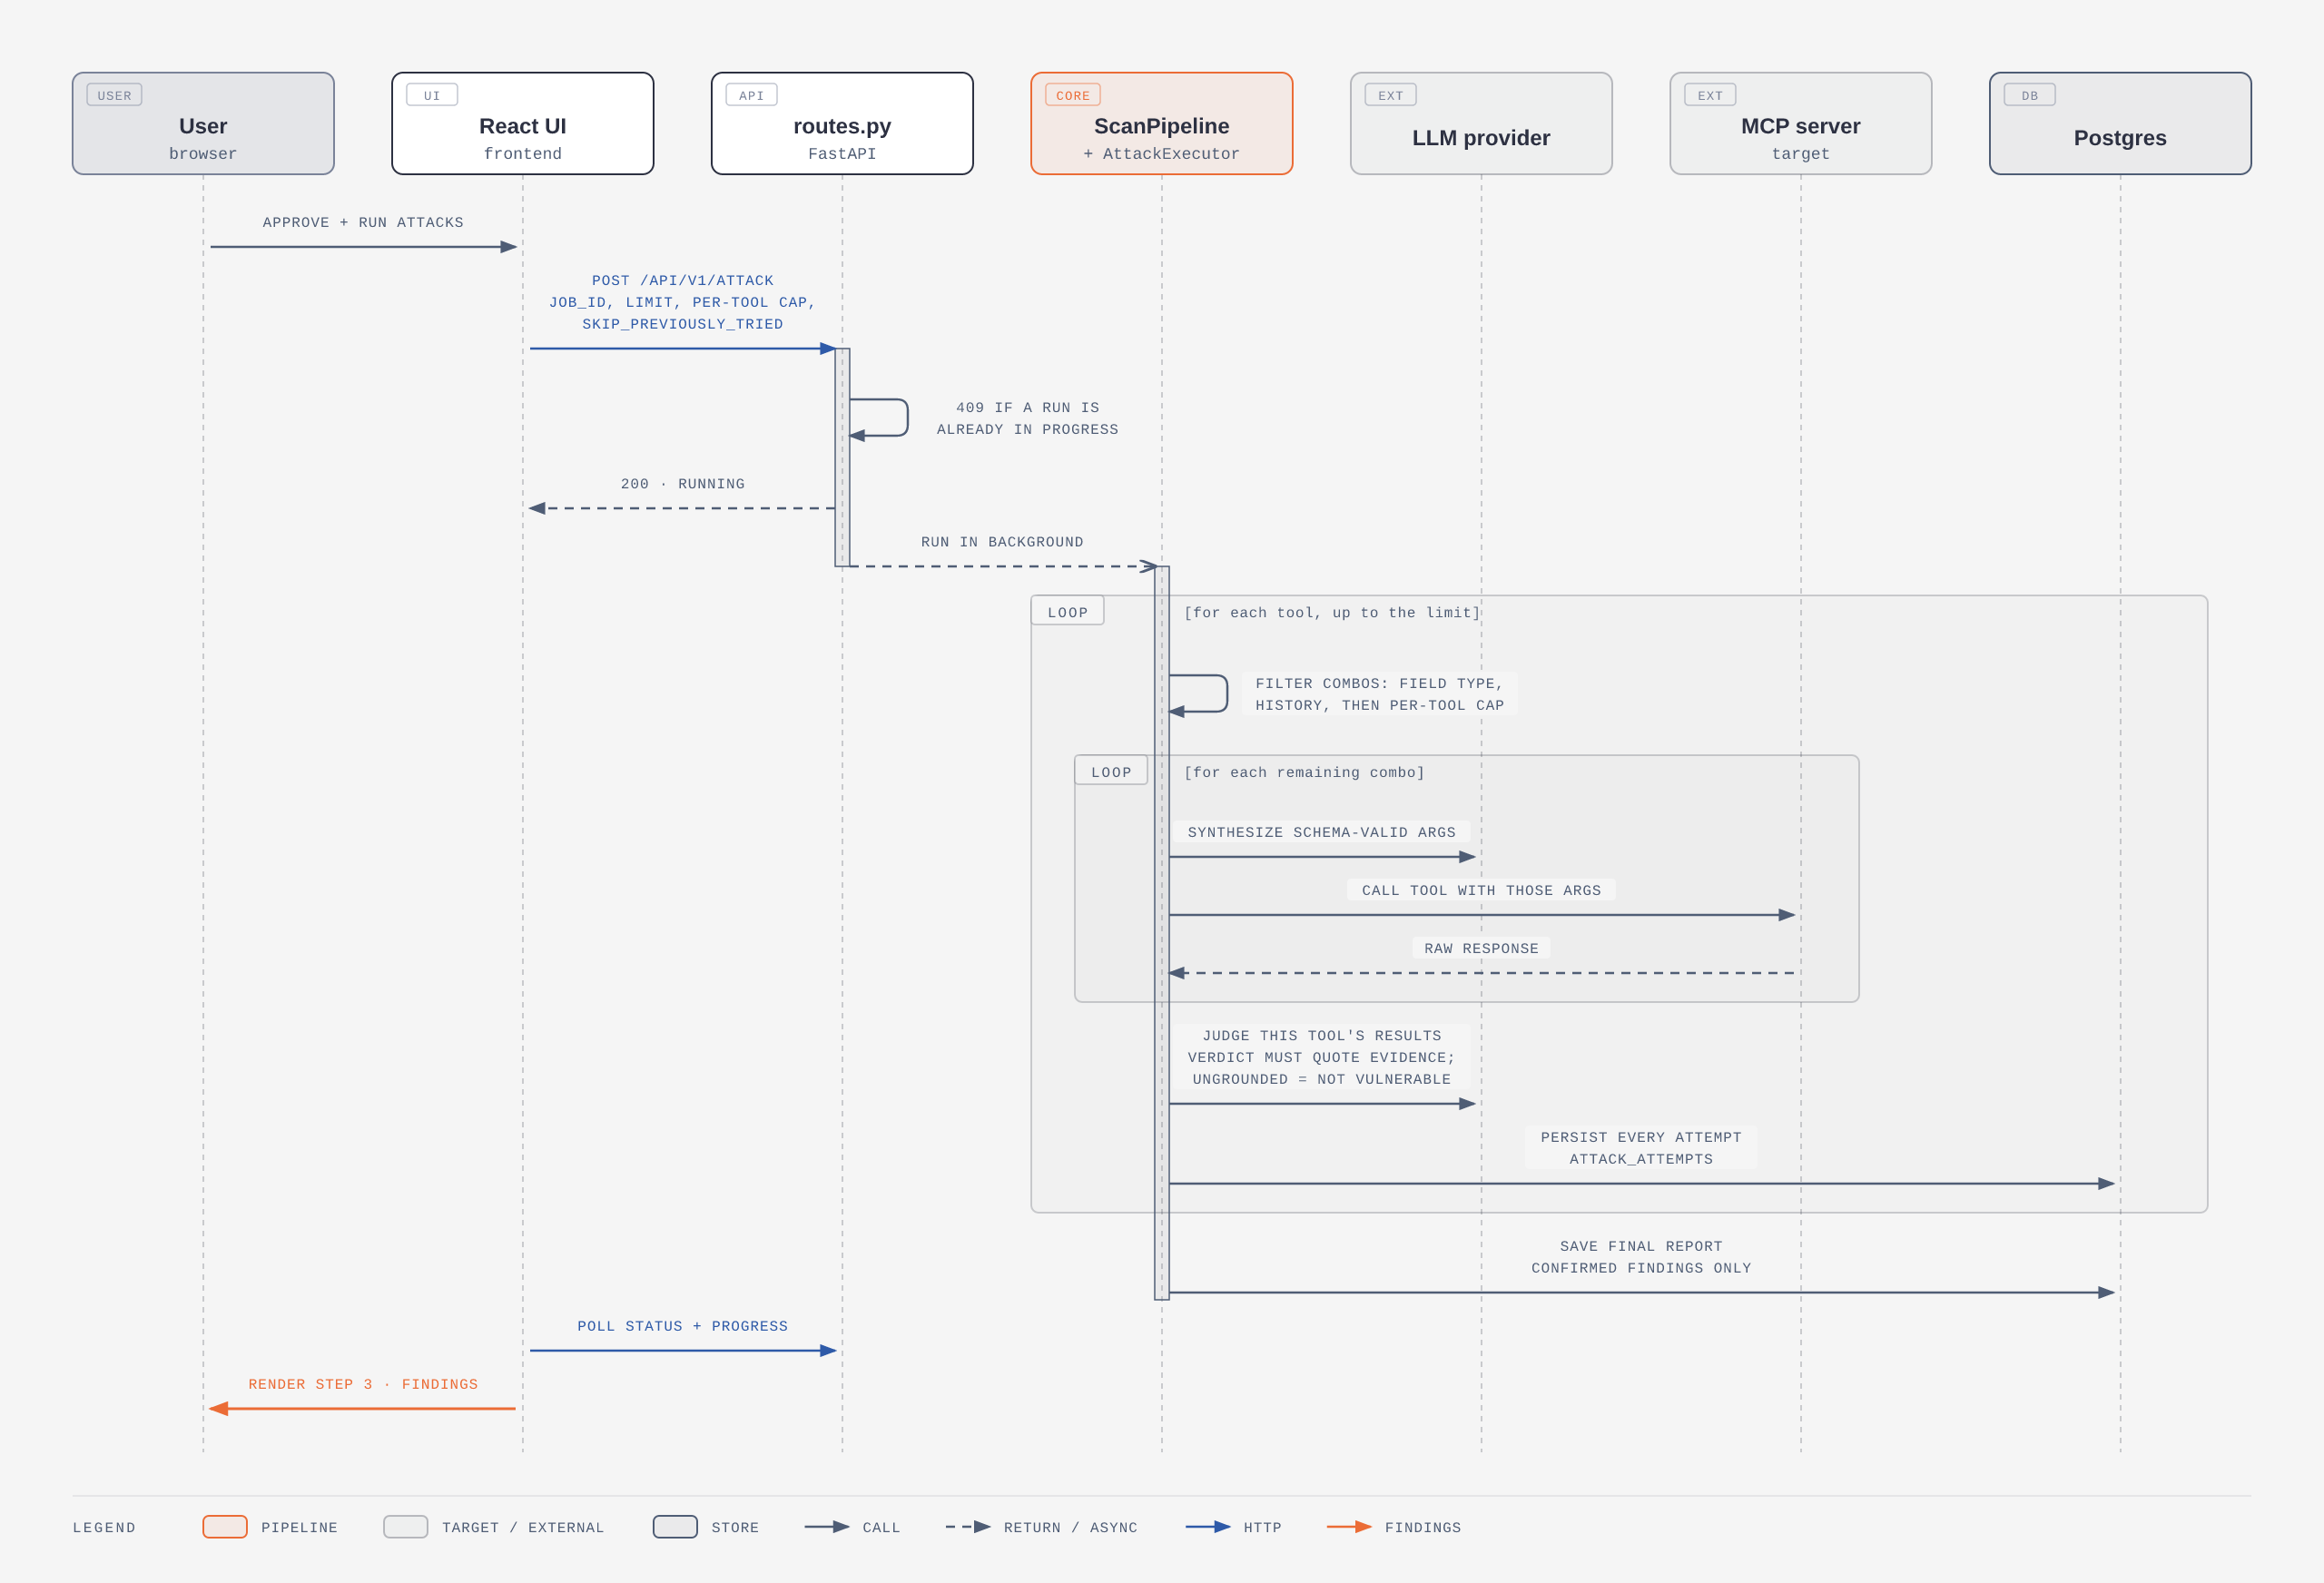
\includegraphics[width=\linewidth]{images/impl-attack-sequence.png}
    \caption{The attack phase: per-tool payload synthesis, live call, and judging.}
    \label{fig:attack-sequence}
\end{figure}

By default a run attacks one tool at a time, which keeps it deterministic and reproducible, the right baseline for measurement. Raising the concurrency cap attacks several tools at once in two phases: the non-timing payloads run concurrently, each tool in its own \gls{mcp} session because one shared session's concurrency safety is not guaranteed, and then the latency-based payloads run serially with nothing else in flight, so load cannot corrupt a timing verdict. The set of findings is the same either way; parallelism changes order and speed, not conclusions.

\section{Dual Evaluation and the Grounded Judge}
\label{sec:evaluator}

Evaluation runs the two checks introduced in Section~\ref{sec:decisions}. The rule-based check matches responses against known-format signatures and latency thresholds; it is fast, free, and precise, but it only sees what it was written to see. The \gls{llm} judge is invoked where semantics are needed, on confirmed rule-based hits for an explanation and a grounded evidence span, and on the categories that are inherently semantic, so the extra model call is spent only where it earns its place.

The judge is constrained rather than trusted. It must return the exact span of the response that proves the leak or the execution, and it is told, per category, that an error, refusal, validation failure, or timeout is a \emph{failed} attack unless the error itself is the disclosure, such as a traceback exposing internal paths or a database error revealing a schema. After the model answers, the code verifies that the quoted span is actually present in the response, normalized for whitespace and case and subject to a minimum length; if the quote is missing, empty, or too short, a ``vulnerable'' verdict is flipped to not-vulnerable, with the original reasoning kept for audit. Because this check is deterministic and model-agnostic, it catches a hallucinated success regardless of which provider or model produced it, while rule-based hits, already grounded in a concrete match, are left untouched.

\section{Authenticated Servers: the OAuth Flow}
\label{sec:oauth}

\gls{mcp} servers exposed over \gls{http} increasingly require \gls{oauth} rather than a static token~\cite{mcp2025spec}. The implementation builds entirely on the official \gls{sdk}'s OAuth client provider, so metadata discovery, \glsdisp{dynamic_client_registration}{dynamic client registration}, and \gls{pkce} are the SDK's responsibility, not reimplemented here. The protocol chain is the standard one~\cite{rfc6749}: the client asks the server which authorization server handles it, asks that server for its endpoints, obtains a client identifier, and completes an authorization-code grant with PKCE~\cite{rfc7636} as mandated for a public client that has no secret to keep confidential.

The flow is matched to a two-phase interface. A start call creates an in-memory connection and begins discovery in the background; its redirect handler opens the system browser to the authorize URL and records the OAuth state so the later callback can be matched to the right pending login. The provider blocks until the callback resolves it with the returned code, the SDK completes the token exchange internally, and discovery and classification then run over the now-authenticated session as the same step. The resulting bearer token is folded into the same process-local credential store every other transport uses, so the attack call needs no OAuth-specific code. Tokens and client information are reused per target \acrshort{url} for the life of the process and are never written to the database or to disk, consistent with the credential posture of Section~\ref{sec:data}.

Two interoperability issues encountered while building this are worth recording, because they are the kind of detail a practitioner repeating the work would hit. One provider, in the absence of an explicit token-endpoint authentication method at registration, defaulted new clients to a confidential-client method and issued a secret the tool had no business holding, after which the SDK sent the client identifier in two places at once and the authorization server rejected it; the fix was to request the public-client method explicitly at registration time. Another provider has no registration endpoint at all, returning a bare 404, which confirmed that dynamic registration is simply unimplemented there and motivated a manual escape hatch that pre-seeds the client information so the SDK skips registration entirely.

\section{Static Analysis Engine}
\label{sec:static-impl}

The static engine reads source and connects to nothing. Source arrives one of two ways, both refusing anything unsafe: a public repository is shallow-cloned over \gls{https} only, with other \acrshort{url} schemes refused and git never prompting for credentials, and then deleted after analysis; an uploaded folder is accepted only for the relevant file types, with absolute paths or paths containing parent-directory references rejected rather than sanitized. A safe file walk applies exclusions, file-count and size caps, and a refusal to follow symlinks out of the root. Figure~\ref{fig:static-flow} shows how a run moves from ingested source to attributed findings.

\begin{figure}[htbp]
    \centering
    % TODO: export images/impl-static-analysis.svg to images/impl-static-analysis.png
    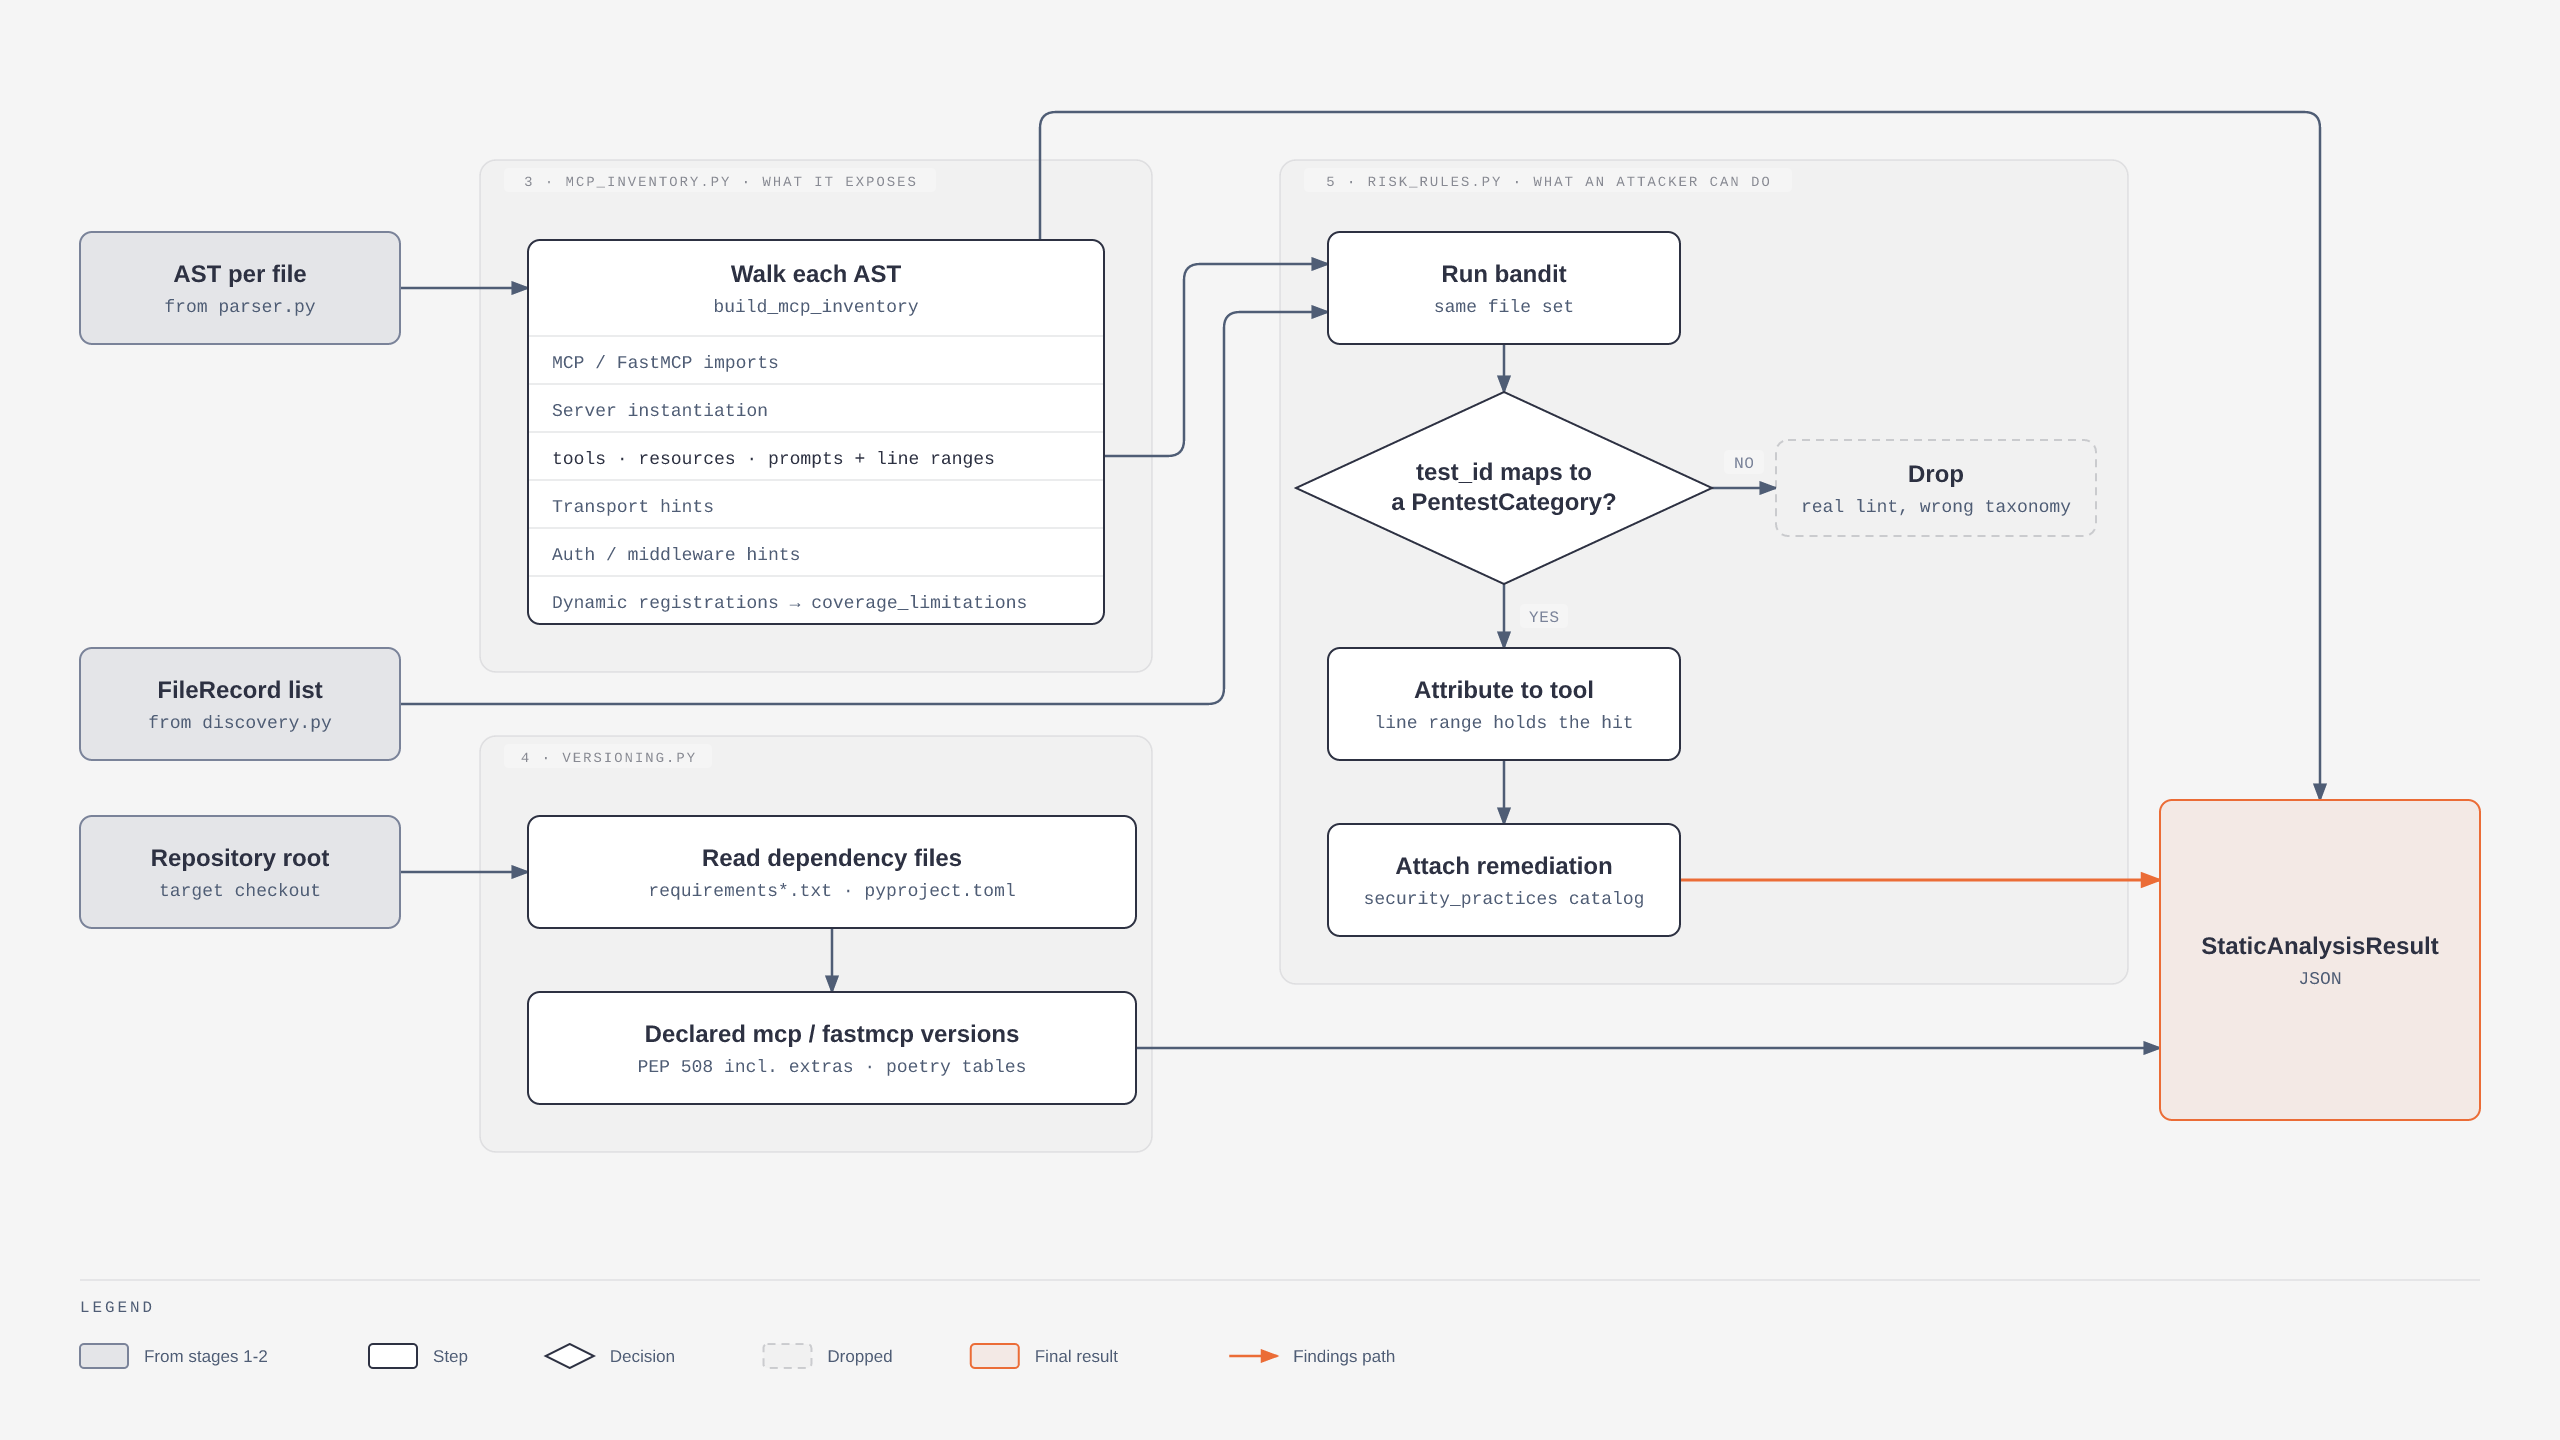
\includegraphics[width=\linewidth]{images/impl-static-analysis.png}
    \caption{Static analysis: parse, inventory the exposed surface, and attribute risk findings to the tool that exposes them.}
    \label{fig:static-flow}
\end{figure}

Each file is parsed to an \gls{ast}, and a syntax error is recorded while the run continues, so analysis is partial rather than all-or-nothing. The inventory pass is hand-written tree walking because it needs MCP-specific knowledge: which function is a registered tool, and where its body ends. It records the registrations with their parameters and line ranges, the transport, and authentication hints, and reads the declared MCP dependency version from the project's requirements. Risk detection reuses Bandit rather than hand-rolling sink matching; this engine's contribution is mapping Bandit's test identifiers onto the taxonomy and attributing each hit to the tool that exposes it. A shell-executing call maps to \gls{command_injection}, a string-built query to \acrshort{sql} injection, a pickle load to \glsdisp{deserialization_attack}{deserialization}, and a hit inside a registered tool's line range is attributed to that tool while a hit outside the taxonomy is dropped. The same analysis is available offline through a command-line entry point, so it can run with neither a server nor the web interface.

\section{Persistence Layer}
\label{sec:persistence}

The database is reached only through a repository component; it is the only code that touches the \gls{orm}, which keeps persistence concerns out of the rest of the pipeline and isolates any future schema change to one place. The \gls{json} columns are written to be portable across both SQLite and PostgreSQL, which is what lets the test suite run the full persistence layer against an in-memory SQLite database and still exercise the same code path production uses, including the round trip from a Pydantic model to a dictionary to database JSON and back that the attack orchestration depends on.

\section{Testing and Continuous Integration}
\label{sec:testing}

The test suite runs without network access. The Jev classifier has no unit tests yet; its behavior is measured instead by the classification benchmark in Chapter~\ref{chap:results}. The earlier \gls{llm} classifier is tested against a stubbed provider, covering the two floor-related failure modes. The persistence layer is tested against in-memory SQLite, including the JSON round trip. The static analysis tests cover both directions of its contribution: a dangerous call inside a registered tool must come back attributed to that tool, and a Bandit finding outside the taxonomy must be dropped rather than reported. A parity test keeps the frontend's copy of the taxonomy in sync with the Python enumerations, and the remediation catalog is checked so that every category resolves to remediation text. 
The same parity check requires every category to carry a valid \gls{cvss} vector, and a deterministic test fixes one known vector, the \gls{sql} injection one, to its expected score of 9.4, its Critical band, and its high, high, low impact, so a change in the library or the catalog cannot silently shift the scores reported in Chapter~\ref{chap:results}.
Continuous integration runs the suite together with Bandit, \texttt{pip-audit}, and \texttt{detect-secrets} on every push, and the latter three currently pass clean against the codebase, verified in CI rather than assumed.
